\documentclass[a4paper,11pt]{amsart}
\usepackage{amssymb}
\usepackage[T1]{fontenc}
\usepackage{indentfirst}
\usepackage{enumerate}
\usepackage{stmaryrd}
\usepackage{xspace}
\usepackage{amsmath}
\usepackage{amsfonts}
\usepackage{url}
\usepackage[colorlinks=true, a4paper=true, pdfstartview=FitV,
linkcolor=blue, citecolor=blue, urlcolor=blue]{hyperref}
\pdfcompresslevel=9

\usepackage[left=2.61cm,right=2.61cm,top=2.72cm,bottom=2.72cm]{geometry}


\usepackage{graphicx}
%%%%%%%for quotes
\usepackage{textcmds}

\usepackage[english,frenchb]{babel}
%\usepackage[latin1]{inputenc}
\usepackage[utf8]{inputenc}
\usepackage{indentfirst, amsfonts, amsmath, amsthm, amssymb, amscd}
\usepackage{amsmath,amsfonts,amscd,bezier}
%%%%%%%%%%%%%%%%%%%%%%%%%
\usepackage[most]{tcolorbox}
%%%%%symbol for EUR
\usepackage{eurosym}
%%%%%%%%
\begin{document}
\begin{tcolorbox}[center,colback=white]
\begin{center}
{\large\textsc{Banknote Authentication}}\\
\end{center}
\end{tcolorbox}

\section{Description}

Central banks incorporate various security features in their banknotes to enable
the general public, retailers, professional cash handlers and central banks to detect
counterfeits. Authenticating whether a banknote is real or not is one of the most common tasks in the banking industry. In this project, we employ classification methods to model the probability that a banknote is genuine or forged, as a function of its features.

\medbreak 

The dataset used in this work at \href{https://archive.ics.uci.edu/ml/datasets/banknote+authentication}{UCI Machine Learning Repository}, which is a repository of freely available datasets. Let us make some comments on the data. These were extracted from images that were taken from genuine and forged banknote-like specimens. For digitization, an industrial camera usually used for print inspection was used. The final images have $400\times400$ pixels. Due to the object lens and distance to the investigated object gray-scale pictures with a resolution of about $660$ dpi were gained. A Wavelet Transform tool was used to extract features from these images. In Section \ref{dataanalysis}, we give more details about the dataset.

\medbreak

Throughout this project, we use Python libraries for the analysis of our dataset as well as for training the machine learning models. More precisely, we use Pandas library to import the dataset, prepare/clean it, and identify the features and the target. For visualizing the dataset we use Searborn library and finally to train machine learning algorithms we use Scikit learn library. Many of the code reproduced herein are adapted from \href{https://machinelearningmastery.com/}{machinelearningmastery.com}.

\medbreak

Now, let us briefly explain how we plan to present our analysis and results. In the first stage, we employ exploratory data analysis to do the data cleaning. We identify the targets and the feature, and visualize their correlations. Then, employ our first classification model: \emph{Logistic Regression}. We work with the data without and with scaling, and then we compare their accuracies. 
We study simple logistic regression, and a regularization problem with $l1$ and $l2$ penalties. The next method employed is the \emph{K-Nearest Neighbor}, where we visualize the confusion matrix, and use K-fold cross validation, and hyperparameter tuning using GridSearchCV to come up with an estimate for the model performance. Then, we employ \emph{Support Vector Machines} with two options, LinearSVC and SVC. We make some plots to visualize some results with different kernels. Our next model employed is \emph{Decision Tree}. Therein, we obtain accuracies results and plot a graphic with a tree to help visualize how the algorithm works. Finally, we employ \emph{Ensemble Methods}. More precisely, we evaluate four different ensemble machine learning algorithms \emph{AdaBoost (AB)} and \emph{Gradient Boosting (GBM)}(Boosting Methods), and \emph{Random Forests (RF)} and \emph{Extra Trees (ET)} (Bagging Methods).

\medbreak

In Section \ref{problem}, we present the formal problem and mention our target audience. In Section \ref{dataanalysis}, we explain the data cleaning, data visualization, and the classification methods used in this project. In Section \ref{results}, we present the key findings of our analysis and discuss the results obtained. Finally, in Section {future}, we discuss about the accuracy of each method, and possible ways to improve them.

\medbreak

Last but not least, we mention that in order to clarify our analysis, and give a clear presentation of the results therein obtained, we add the notebook file to this report. In this way, the reader can easily follow the graphics and ideas described in this project.

\section{Problem Statement \& Target Audience}\label{problem} 

Our goal is to predict whether a banknote is genuine or forged. Banknote authentication stays an important challenge for the central banks in order to keep the strength of the financial system around the world. One of the most substantial tasks is to find counterfeit banknotes.  

\medbreak

In general, people cannot feel whether a banknote is fake or genuine. For example, 
blind and partially sighted people are not able to know both the value and authenticity of banknotes, since there is no available method for them to check for the authenticity and for forgeries the banknotes. But even people without visualization difficulties cannot easily identify the authenticity of a banknote, since these forgery and genuine banknotes are typically equal. 

\medbreak

Our target is the general public, retailers, professional cash handlers and central banks.

\section{Data Analysis}\label{dataanalysis}

We begin our analysis by getting the dataset, which is available at \href{https://archive.ics.uci.edu/ml/datasets/banknote+authentication}{UCI Machine Learning Repository}. It contains data on images taken from genuine and forged banknote-like specimens. The number of instances (rows) in the data set is $1372$, and the number of variables (columns) is $5$.

Features such as wavelet variance, wavelet skewness, wavelet kurtosis, and image entropy are extracted from the images.

\medbreak

The features (input variables), which are all of quantitative type, are given by
\begin{flushleft}
\emph{Variance of Wavelet Transformed Image}\\    
\emph{Skewness of Wavelet Transformed Image}\\
\emph{Curtosis of Wavelet Transformed Image}\\
\emph{Entropy of Image}\\
\end{flushleft}
and the target/response (output variable), which is also of qualitative type, is given by
\begin{flushleft}
\emph{Class},
\end{flushleft}
which has two outcomes: $1$ stands for \textbf{genuine}, and $0$ stands for \textbf{forged} banknotes.  

\medbreak

Once we identify the types of our features we proceed to our next stage: Data Cleaning. Therein, we check for missing values, change headers of columns, observe the frequency of the outcomes, and plot a \emph{pairplot} graphic to visualize the relationship among all columns of the dataset (features and target). To better understand the correlations among the terms in our study, we use a heatmap. Then, we create the feature matrix $X$, and the response vector $y$. 

\medbreak

\noindent{\textsc{Logistic Regression}.} We consider the simple case, and the regularization problem with $l1$ and $l2$ penalties. In general, these methods are sensitive to outliers, so we use the \emph{IsolationForest} method to detect anomalies. Next, we standardize the data using \emph{StandardScaler}. We use a train/test split with a test size of $20\%$ of the original data.  As soon as the data is cleaned and prepared, we use the necessary methods from sklearn.

\medbreak

\noindent{\textsc{K-Nearest Neighbor}.} With this algorithm, we use another method for scaling the data, and another one for removing the outliers, \emph{MaxAbsScaler}, and \emph{LocalOutlierFactor}, respectively. Again, we use a train/test split with a test size of $20\%$ of the original data. In this way, after removing the outliers the training set has 1092 samples in the range of $-1$ and $1$. Then, we obtain the accuracy results and plot the confusion matrix. To obtain another estimate of the model performance, we use \emph{K-Fold Cross Validation} and hyperparameter tuning using \emph{GridSearchCV}.

\medbreak

\noindent{\textsc{Support Vector Machines}.} We use the \emph{One-Class SVM} to capture the density of the majority class and classify examples on the extremes of the density function as outliers, and normalize the feature matrix with the help of \emph{Normalizer}. Then, we obtain the accuracy of SVM with different kernels, and to visualize the support vectors we come back to the data without scaling.

\medbreak

\noindent{\textsc{Decision Tree}.} As throughout our project, we scale the feature matrix, and remove the outliers. Before going into the method itself, we obtain that the number of nodes is $45$ and the maximal depth is $7$. Next, we establish the accuracy on the trainning and test (validation) sets, and visualize the tree.

\medbreak

\noindent{\textsc{Ensemble Methods}.} We evaluate four different ensemble machine learning algorithms:
\begin{flushleft}
\textbf{Boosting Methods:} \emph{AdaBoost (AB) and Gradient Boosting (GBM).}\\
\textbf{Bagging Methods:} \emph{Random Forests (RF) and Extra Trees (ET).}
\end{flushleft}

\section{Key Findings}\label{results}

Let us begin with the exploratory data analysis. There aren't any missing entry and the outcomes have a frequency of $762$ values for class \textbf{0}, and $610$ values for class \textbf{1}. the feature that has the biggest correlation with the target is \emph{Curtosis of Wavelet}, with a value of $0.156$. 

Our accuracy results for Logistic Regression can be summarised in the following table.
\begin{table}[h!]
  \begin{center}
    \caption{\textsc{Logistic Regression}}
    \label{tab:table1}
    \begin{tabular}{l|c|c|r|} 
      & \textsc{log-reg} & \textsc{$l1$-penalty} & \textsc{$l2$-penalty}\\
      \hline
      \textsc{precision} & 97.83\%  & 98.18\% & 98.18\%\\
      \textsc{recall} & 97.81\% & 98.18\% & 98.18\%\\
      \textsc{f1-score} & 97.81\%  & 98.18\% & 98.18\%\\
      \textsc{accuracy} & 97.81\% & 98.18\% & 98.18\%\\
      \textsc{auc} & 97.86\% & 98.19\% & 98.19\%\\
    \end{tabular}
  \end{center}
\end{table}
Observe that Logistic Regression with a penalty gives a better accuracy of $98.18\%$ for predicting whether a banknote is a forgery or authentic. 

\medbreak

The K-Nearest Neighbor algorithm with the number of neighbors in the range between $2$ and $19$ gives an accuracy and $f1$ scores of 100\% in the validation set with $275$ samples, which is excellent. The following confusion matrix is obtained:
\begin{table}[h!]
  \begin{center}
    \caption{\textsc{K-NN Confusion Matrix}}
    \label{tab:table2}
    \begin{tabular}{l|c|r|} 
      & \textsc{False} (Ground Truth) & \textsc{True} (Ground Truth)\\
      \hline
      \textsc{True} (Prediction) & 148 & 0\\
      \textsc{False} (Prediction) & 0 & 127\\
    \end{tabular}
  \end{center}
\end{table}

\medbreak

In order to obtain an estimate of the model performance in the whole data we employ K-Fold Cross Validation and GridSearchCV. We then obtain the following accuracy results.
\begin{table}[h!]
  \begin{center}
    \caption{\textsc{Accuracy}}
    \label{tab:table3}
    \begin{tabular}{l|c|r|} 
      & \textsc{GridSearchCV}  & \textsc{F-Fold Cross Validation}\\
      \hline
      \textsc{K-NN}& 99.85\% & 99.85\%\\
    \end{tabular}
  \end{center}
\end{table}

\medbreak

The \emph{Support Vector Machine} algorithms gives the following accuracy results.
\begin{table}[h!]
  \begin{center}
    \caption{\textsc{Accuracy of SVC with Kernel}}
    \label{tab:table4}
    \begin{tabular}{l|c|c|c|c|r|} 
      & \textsc{linear}  & \textsc{poly} & \textsc{rbf} & \textsc{sigmoid}\\
      \hline
      \textsc{SVC}& 99.63\% & 99.63\% & 99.63\% & 90.54\%\\
    \end{tabular}
  \end{center}
\end{table}

Observe that the use of a \emph{sigmoid} kernel implies in a drastically loss of accuracy. Next, we visualize the decision boundaries of two features. Recall that wee do not scale our data since we want to plot the support vectors.

\pagebreak

\begin{figure}
 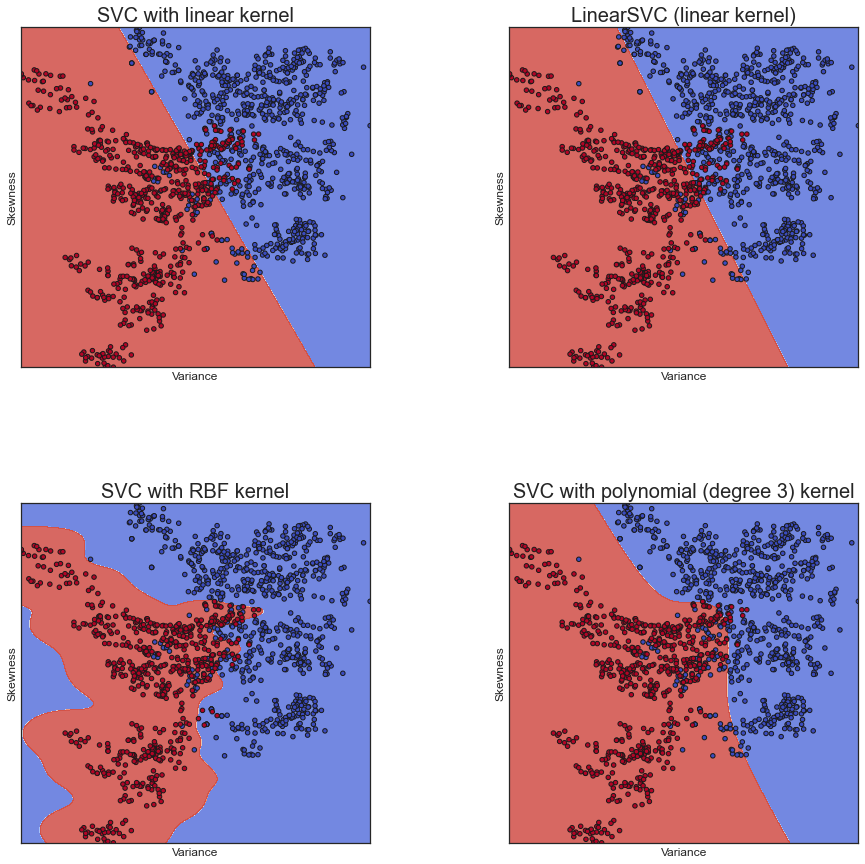
\includegraphics[width=\linewidth]{download.png}
  \caption{Decision Boundaries}
  \label{fig:svc1}
\end{figure}

\medbreak

In regard with \emph{Decision Tree}, we do not investigate an optimal value for the number of nodes and maximal depth, which can be done by using cross validation. In our analysis, we obtain that the number of nodes is $45$ and the maximal depth is $7$.
\begin{table}[h!]
  \begin{center}
    \caption{\textsc{Accuracy of Decision Tree}}
    \label{tab:table5}
    \begin{tabular}{l|c|r|} 
      & \textsc{Training Set}  & \textsc{Validation Set}\\
      \hline
      \textsc{accuracy}& 100\% & 99.27\%\\
      \textsc{precision}& 100\% & 98.31\%\\
      \textsc{recall} & 100\% & 100\%\\
      \textsc{f1-score} &100\% & 99.15\%\\
    \end{tabular}
  \end{center}
\end{table}

\medbreak 

Next, we visualize the decision tree algorithm in action.

\pagebreak 

\begin{figure}
 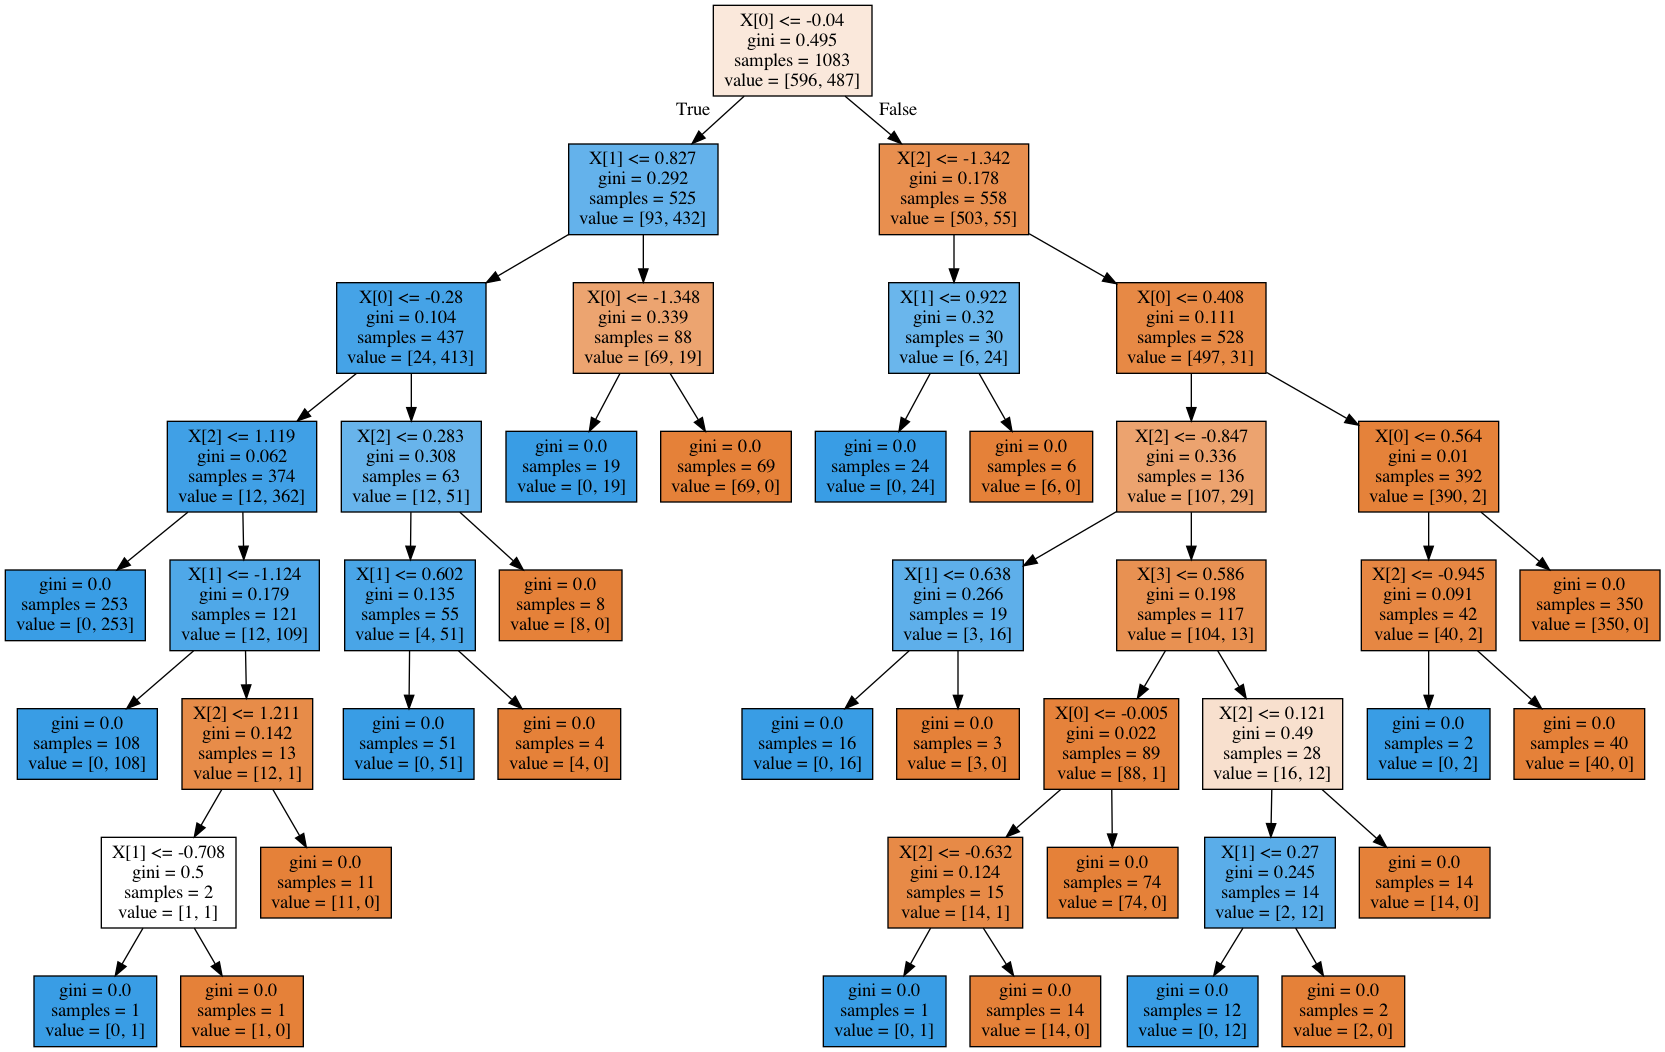
\includegraphics[width=1.15\columnwidth]{bank_note_tree.png}
  \caption{Decision Boundaries}
  \label{fig:dsb}
\end{figure}

\medbreak

Finally, by employing \emph{Ensemble Methods} we obtain the following results.
\begin{table}[h!]
  \begin{center}
    \caption{\textsc{Ensemble Methods}}
    \label{tab:table6}
    \begin{tabular}{l|r|} 
      & \textsc{Accuracy}\\
      \hline
      \textsc{AdaBoostClassifier}& 99.25\% \\
      \textsc{GradientBoostingClassifier}& 99.44\%\\
      \textsc{RandomForestClassifier} & 95.53\%\\
      \textsc{ExtraTreesClassifier} & 99.72\%\\
    \end{tabular}
  \end{center}
\end{table}

\medbreak

This suggests that ExtraTreesClassifier may be worthy of further study.

\section{Final Comments}\label{future}

The accuracy obtained in each method is quite amazing. It gives us a range between $97.81\%$ and $100\%$ (on 275 validation samples). At this point we should ask ourselves what to do to improve our results. As is common practice, it is natural to ask what happens when we work with more samples. Maybe a number of samples around $10.000$ would be a good starting point. then, we would dive into a more challenging analysis.

\medbreak

Removing outliers was essential in our accuracies, since the methods herein employed are sensitive to them. So, a natural problem is to understand their natures and theirs relationship with the features. for instance, when using Logistic Regression with IsolationForest we dropped 110 samples in a total of 1097 training samples. What do they represent? The reduction of outliers in the other methods are not so big. This leaves us with a thought: Let's then dive into other classification methods. 

\medbreak

To better understand the decision boundaries among the features, we could plot several graphics involving each one of the features. Recall that in our analysis we only picked two features. In regard with Decision Trees, we believe there is room for improvement, since in our analysis we did not focus on finding the optimal parameters for number of nodes and maximal depth. This can be done without much trouble by using cross validation.

\medbreak

Finally, concerning Ensemble Methods we obtained pretty good accuracy results. One starting point for further studies could be a more careful analysis of each method, in particular ExtraTreesClassifier, which gave us the best score. 
\end{document}